\chapter{Greedy}
\section{Enun't}
\myindent
Se citesc 3 numere naturale S, n 'si e cu urm'atoarele semnifica'tii: S este o sum'a de bani care trebuie pl'atit'a folosind bancnote care au valori puterile lui e de la 1 la $e^{n}$. S'a se afi'seze la final num'arul de bancnote folosite. Datele se vor citi din fi'sierul Euro.in.\\

Sursa problemei -$>$ \cite{Greedy}
\vspace{5mm}
\section{Descrierea solu'tiei problemei}
\myindent
Pentru rezolvarea acestei probleme se poate opta pentru o variant'a scurt'a 'si simpl'a. Se 'incearc'a aflarea valorii maxime a unei bancnote printr-o iterare de la 0 p\^an'a la puterea maxim'a. Dup'a aflarea valorii maxime va trebui s'a se aplice un concept Greedy foarte simplu pentru minimizarea num'arului de bancnote. Se pl'ate'ste mai 'int\^ai c\^at se poate cu bancnote de valoare maxim'a, apoi c\^and nu se mai poate, se va pl'ati restul sumei cu bancnote a c'aror valoare e din ce 'in ce mai mic'a p\^an'a c\^and suma este pl'atit'a. Se poate afla foarte usor num'arul de bancnote printr-o 'imp'artire a sumei la valoarea maxim'a, num'arul fiind dat de c\^at. Restul va fi pl'atit cu bancnote mai mici. Dup'a ce s-a efectuat plata se va afi'sa rezultatul.

\newpage
\section{Prezentarea algoritmului de rezolvare a problemei}
\begin{lstlisting}[language=Python]
int main()
	citire sum;
	citire max_pow;
	citire baza;

	max = 1;
	nr = 0;

	pentru i de la 0 la max_pow - 1
		daca(max * baza > sum)
			inchide for-ul;

		max = max * baza;

	cat timp sum > 0
		nr = nr + sum / max;
		sum = sum % max;
		max = max / baza;

	scrie nr;
\end{lstlisting}

\vspace{10mm}
\section{Aprecierea complexit'a'tii algoritmului propus}
\myindent
Din punct de vedere temporal, programul con'tine un for de la 0 la max\_pow care va face 'in cel mai r'au caz max\_pow pasi, deci O(max\_pow) 'si un while care depinde de sum'a. Num'arul de itera'tii va depinde de puterea bazei la valoarea maxim'a pe care o poate avea o bancnot'a, adic'a va depinde de num'arul de tipuri de bancnote pe care le avem la dispozi'tie, deci avem complexitate O($log_{baza}max$). Astfel complexitatea final'a va fi O(max\_pow + $log_{baza}max$.

\section{Analiz'a succint'a asupra posibilit'a'tii de ob'tinere a optimului global}
\myindent
Algoritmul respect'a proprietatea de substructur'a optimal'a deoarece solu'tia subproblemei, adic'a num'arul de bancnote pentru un tip ajut'a al rezolvarea problemei, adic'a num'arul total de bancnote. De asemenea, algoritmul respect'a si proprietatea de alegere de tip Greedy deoarece nu se calculeaz'a num'arul bancnotelor pe baza valorilor anterior calculate.

\section{Exemplificarea aplic'arii algoritmului propus pentru un exemplu sugestiv}
\subsection{Exemplu de input}
\begin{verbatim}
Euro.in
444 5 2

Rezultat: 16
\end{verbatim}

\subsection{Aplicarea algoritmului}

\begin{figure}[H]
\centering
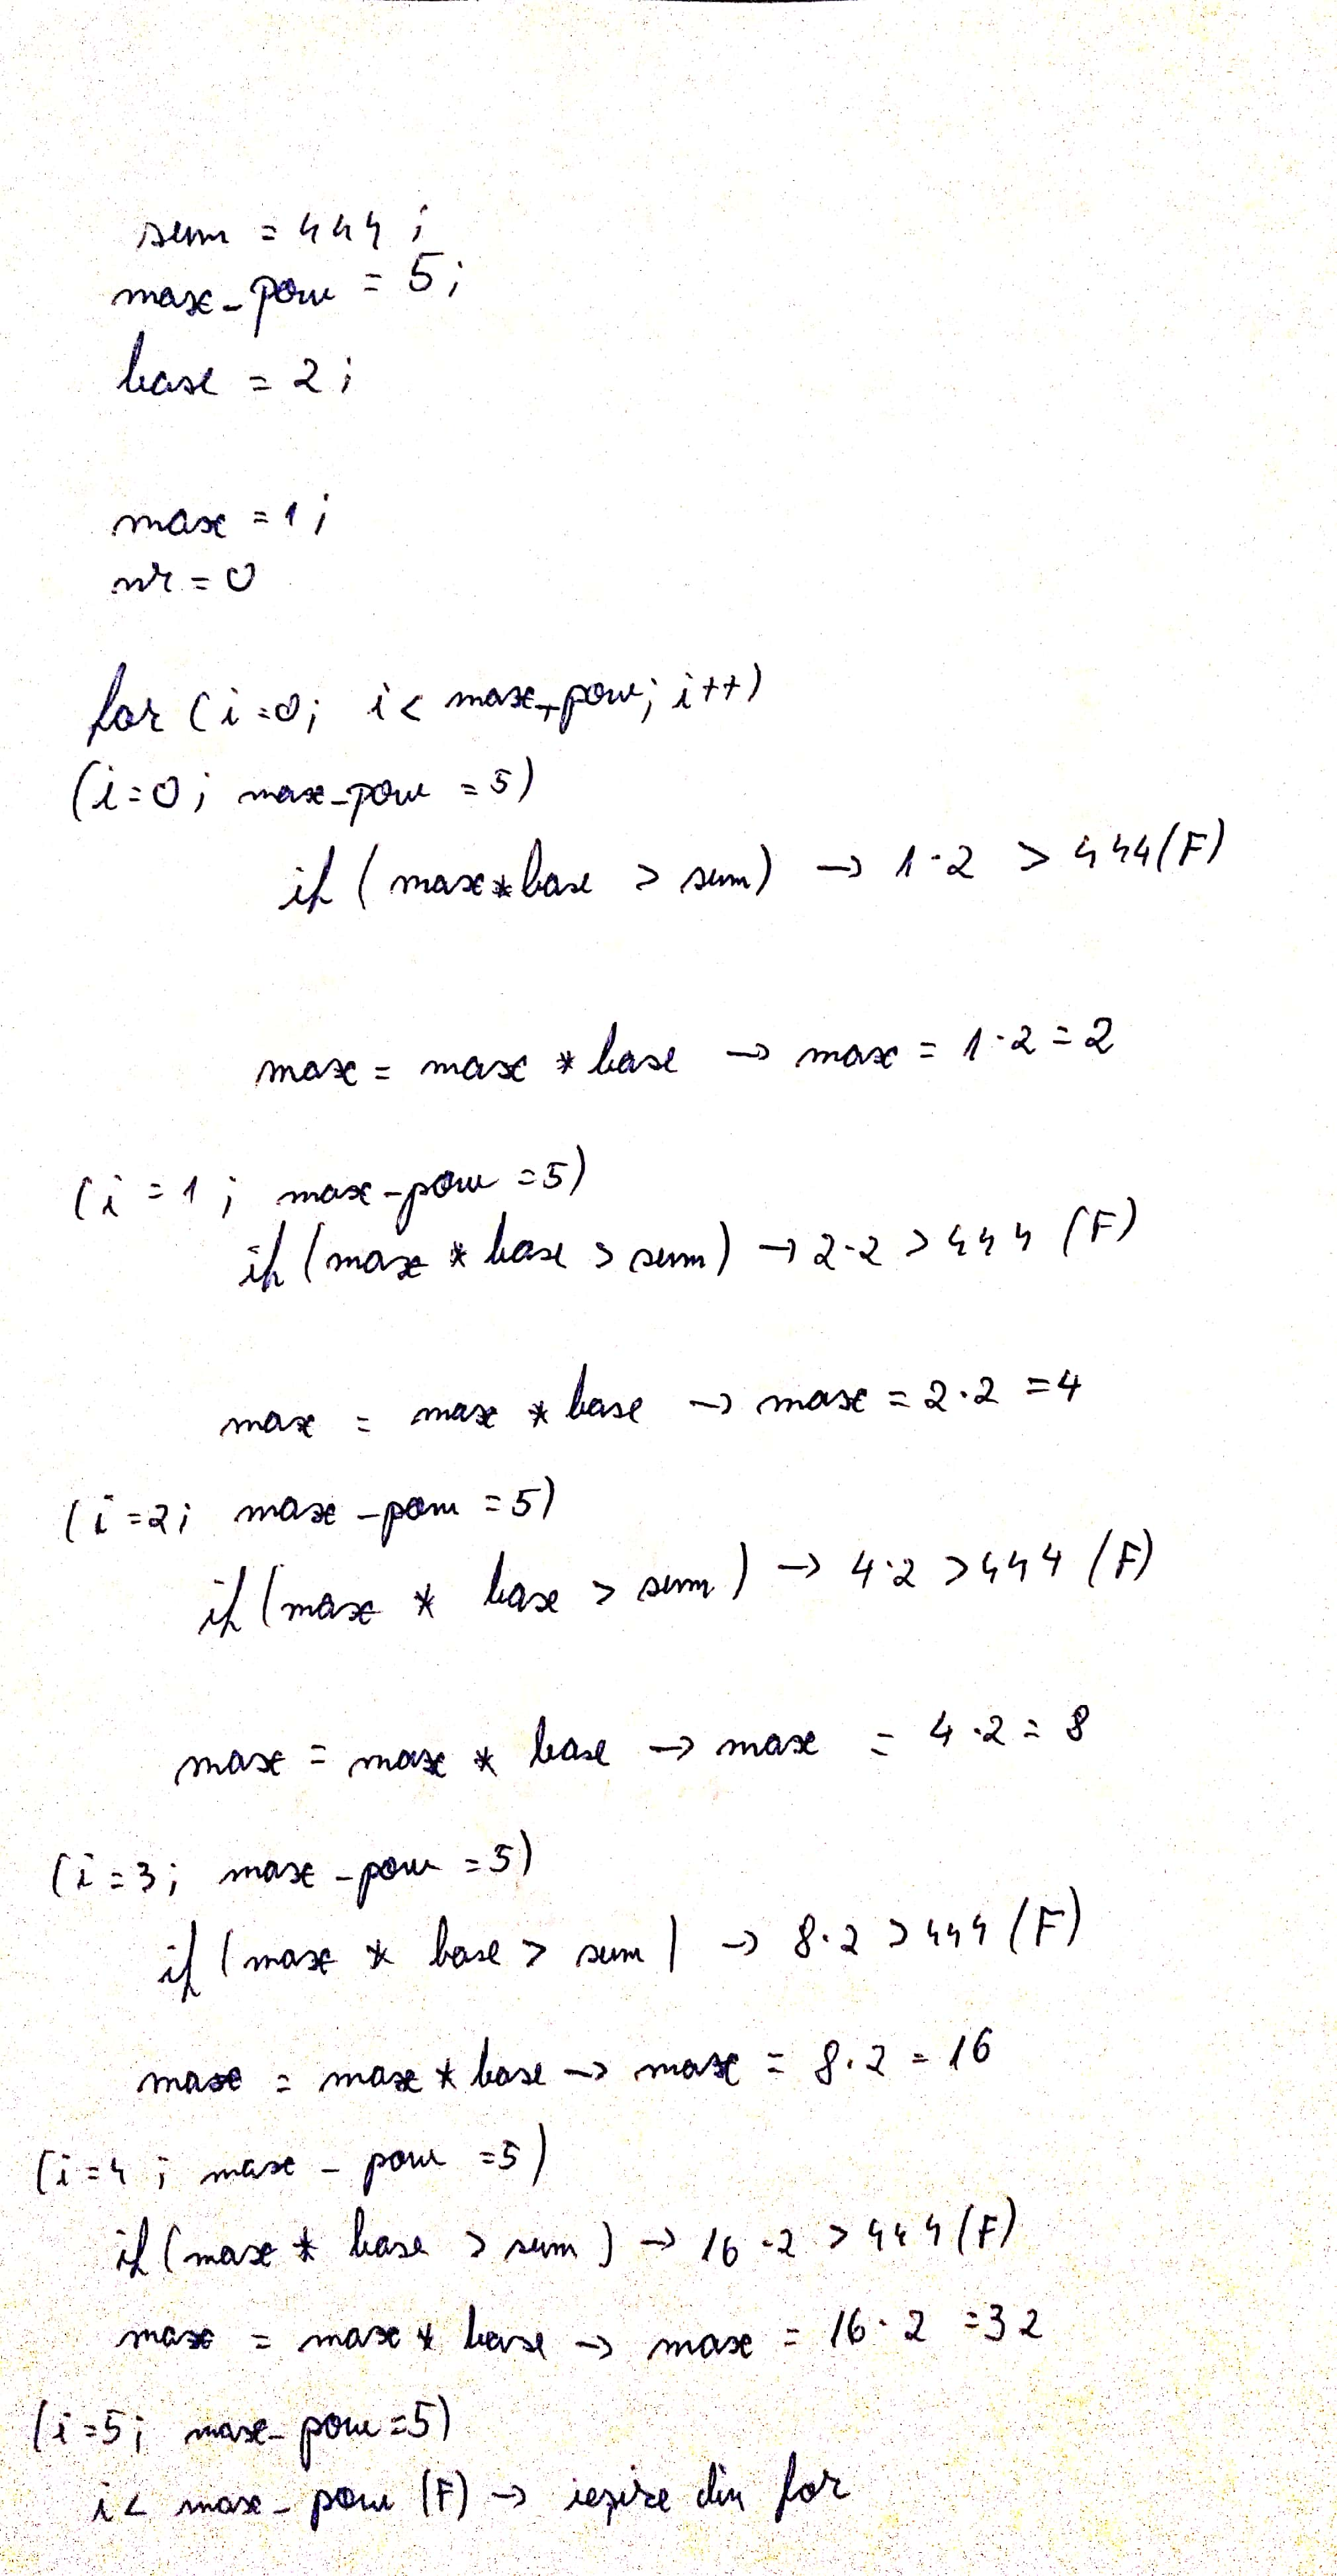
\includegraphics[scale = 0.12]{Greedy/for}
\end{figure}

\vspace{5mm}
\myindent
Algoritmul 'incepe prin citirea parametrilor 'si intrarea 'in for care stabile'ste valoarea maxim'a a unei bancnote 'in func'tie de puterea maxim'a 'si 'in func'tie de sum'a. Practic, fiecare itera'tie din for va verifica urm'atoarea putere a bazei, astfel va ie'si puterea cea mai mare.

\begin{figure}[H]
\centering
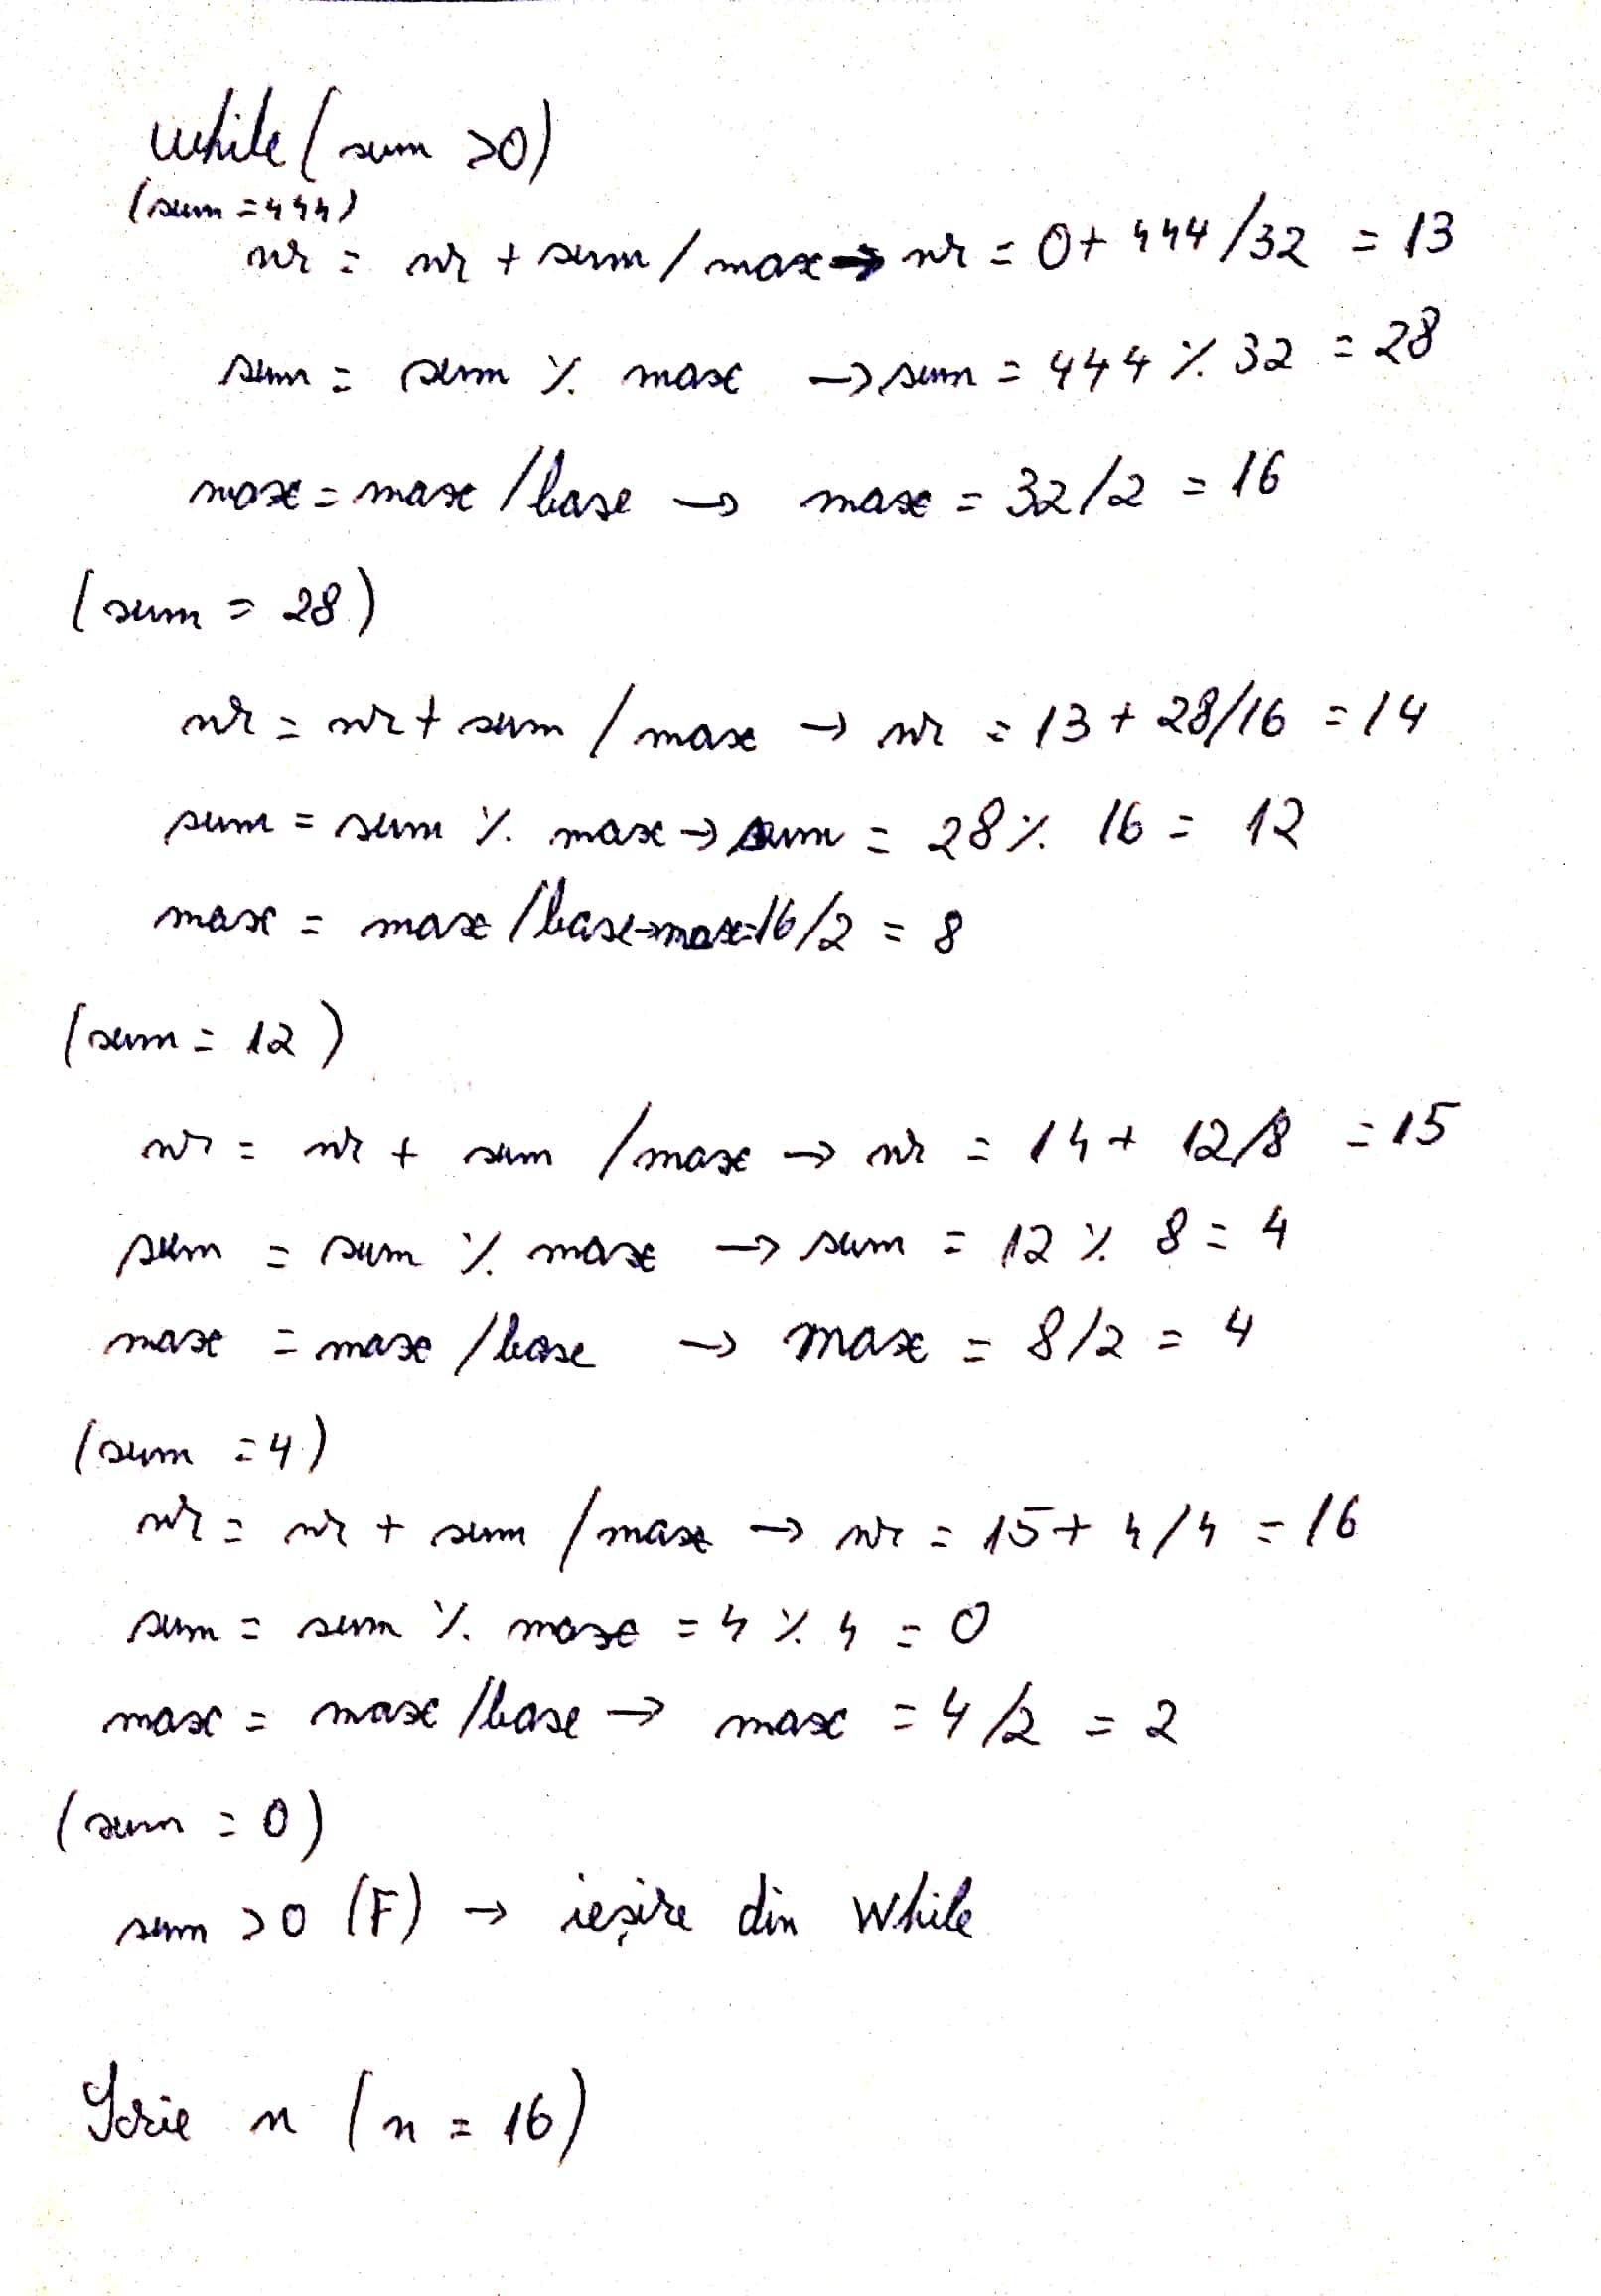
\includegraphics[scale = 0.2]{Greedy/while}
\end{figure}
\myindent
Dup'a g'asirea maximului se va itera prin while-ul care va scoate num'arul de bancnote. Aici se va 'imp'ar'ti suma la valoarea maxim'a 'si va folosi: c\^atul ca s'a numere bancnotele folosite 'si restul c\^atului pentru restul de plat'a. La urm'atoarea itera'tie se va num'ara c\^at din restul r'amas se poate pl'ati cu bancnote cu urm'atoarea valoare maxim'a si tot a'sa. 'In final, dup'a ce se pl'ate'ste toat'a suma, while-ul se 'incheie 'si se afi'seaz'a num'arul de bancnote.